\documentclass{report}
\title{CS245 Course Notes}
\author{mzx!}
\date{\today}
\newcommand{\ibx}[1]{\framebox[1.1\width]{ #1 }}
\usepackage{amsmath,amssymb}
\usepackage{hyperref}
\usepackage{enumitem} 
\hypersetup{
    colorlinks,
    citecolor=black,
    filecolor=black,
    linkcolor=black,
    urlcolor=black
}

\PassOptionsToPackage{svgnames}{xcolor}
\usepackage{tcolorbox}
\usepackage{lipsum,xcolor,color}
\tcbuselibrary{skins,breakable}
\usetikzlibrary{shadings,shadows}

\definecolor{title_color}{HTML}{ea7dc7}
\definecolor{back_color}{HTML}{f7e8e8}

\newcounter{defboxctr}
\newenvironment{defbox}{%
\refstepcounter{defboxctr}% increment the environment's counter
    \tcolorbox[beamer,%
    noparskip,breakable,
    colback=back_color,colframe=title_color,%
    title={Definition \thedefboxctr}]}%
    {\endtcolorbox}
    \numberwithin{defboxctr}{section}






\newcommand{\iep}[0]{$\mathcal{I} \vDash_E \varphi$ }
\newcommand{\niep}[0]{$\mathcal{I} \nvDash_E \varphi$ } 
\newcommand{\vfi}[0]{$\varphi$ }
\newcommand{\vmi}[0]{$\mathcal{I}$ }
\newcommand{\ee}[0]{environment $E$ }
\newcommand{\ii}[0]{Interpretation \vmi }



\begin{document}
\maketitle
\tableofcontents
\chapter{TBD}
\section{Satisfaction of predicate formulas}
\begin{defbox}
An interpretation $\mathcal I$ and enviroment $E$ \textbf{satisfy}  a formula $\varphi$, denoted $\mathcal I\vDash_E \varphi$ if $\varphi^{{\mathcal I},E} = T$\\
They \textbf{do no satisfy} $\varphi$ ($\mathcal I\nvDash \varphi$) if $\varphi^{{\mathcal I},E} = F$
\end{defbox}
\subsection{Satisfaction Relation}
We define the \textbf{Satisfaction Relation} $\mathcal{I} \vDash_E \varphi$ recursively defined as follows:
\begin{itemize}
\item If \ibx{$\varphi = P(t_1,...,t_n)$} for a predicate $P$ and terms $t_1,t_2,t_3,...,t_n$\\
$\mathcal{I}\vDash_E \varphi\iff\langle{t_1^{\mathcal{I},E}},...,{t_n^{\mathcal{I},E}}\rangle\in P^\mathcal{I}$\\In other words,$\mathcal{I}$ and $E$ satisfy $P(t_1,...,t_n)$ if the terms $t_i$ under $\mathcal{I}$ and $E$ correspond to values in the domain that satisfy the predicate $P$ under $\mathcal{I}$
\item If \ibx{$\varphi = (\neg \alpha)$}, then \iep $\iff \mathcal{I} \nvDash_E \alpha$
\item If \ibx{$\varphi = (\alpha \land \beta)$}, then \iep $\iff\mathcal{I} \vDash_E \alpha\text{ and }\mathcal{I} \vDash_E \beta$
\item If \ibx{$\varphi = (\alpha \lor \beta)$}, then \iep $\iff\mathcal{I} \vDash_E \alpha\text{ or }\mathcal{I} \vDash_E \beta$ or both
\item If \ibx{$\varphi = (\alpha \to \beta)$}, then \iep $\iff\mathcal{I} \nvDash_E \alpha\text{ and }\mathcal{I} \vDash_E \beta$ or both
\item If \ibx{$\varphi = (\forall x\alpha)$}, then \iep $\iff$ for every $a\in D^\mathcal{I}$, we have $\mathcal{I}\vDash_E[x\to\alpha]\alpha$
\item If \ibx{$\varphi = (\exists x\alpha)$}, then \iep $\iff$ there is some $a\in D^\mathcal{I}$, we have $\mathcal{I}\vDash_E[x\to\alpha]\alpha$
\end{itemize}
If \iep for every environment $E$, then $\mathcal{I}$ \textbf{Satisfy} $\varphi$ and we write $\mathcal{I} \vDash\varphi$ 
\subsection{Valid}
\begin{defbox}
A formula \vfi is
\begin{itemize}
\item \textbf{Valid} if \iep for ever interpretation \vmi \textbf{and} every \ee
\item \textbf{Satisfiable} if \iep  for some \ii and \ee
\item \textbf{Unsatisfiable} if \niep  for every \ii and \ee
\end{itemize}
\end{defbox}
\paragraph{Show Entailment DOES Hold} For example $a\vDash b$, then assume a is true and b is false\ibx{seek for \textbf{contradiction} }
\paragraph{Show Entailment DOES NOT Hold} For example $a\nvDash b$, then show that \ibx{a is true AND b is false}\\
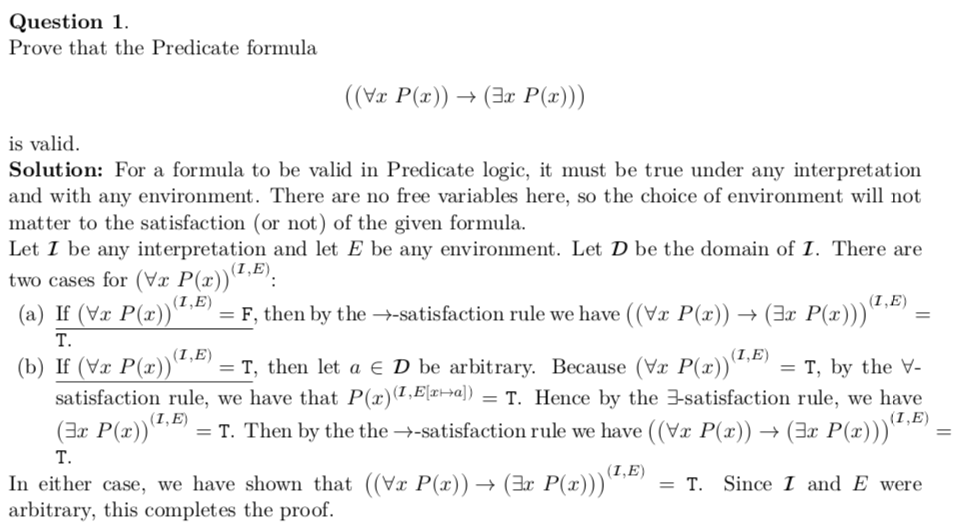
\includegraphics[width=\textwidth]{ex1} 

Not FINISHED

\section{Natural Deduction for Predicate Logic}

\begin{defbox}
$${{(\forall x \alpha)}\over {a[t/x]}}\forall e$$
if we have a formula $(\forall x \alpha)$, then we can conclude that we can substitute anything for $x$ in $\alpha$
\end{defbox}
\begin{defbox}
$${{a[t/x]}\over {(\exists x \alpha)}}\exists i$$

\end{defbox}


\chapter{Soundness and Completeness}
\section{Soundness}
\begin{defbox}
A proof system is \ibx{sound} if whenever $\sum \vdash\varphi$, then $\sum \vDash\varphi$
\end{defbox}
Soundness says that if we have a proof in our proof system, then it says something about the relationship of the formulas involved under all valuations
\begin{defbox}
A proof system is \ibx{complete} if whenever $\sum \vDash\varphi$, then $\sum \vdash\varphi$
\end{defbox}
\chapter{Index}
\paragraph{Predicate} Relation
\end{document}
